\documentclass{article}

% if you need to pass options to natbib, use, e.g.:
%     \PassOptionsToPackage{numbers, compress}{natbib}
% before loading neurips_2021

% ready for submission
%\usepackage{neurips_2021}

% to compile a preprint version, e.g., for submission to arXiv, add add the
% [preprint] option:
\PassOptionsToPackage{numbers}{natbib}
\usepackage[preprint]{neurips_2021}

% to compile a camera-ready version, add the [final] option, e.g.:
%\usepackage[final]{neurips_2021}

% to avoid loading the natbib package, add option nonatbib:
%    \usepackage[nonatbib]{neurips_2021}

\usepackage[utf8]{inputenc} % allow utf-8 input
\usepackage[T1]{fontenc}    % use 8-bit T1 fonts
\usepackage{hyperref}       % hyperlinks
\usepackage{url}            % simple URL typesetting
\usepackage{booktabs}       % professional-quality tables
\usepackage{amsfonts}       % blackboard math symbols
\usepackage{nicefrac}       % compact symbols for 1/2, etc.
\usepackage{microtype}      % microtypography
\usepackage{xcolor}         % colors
\usepackage{graphicx}
\graphicspath{ {images/} }
\usepackage{booktabs}
\usepackage{csvsimple}


\title{The Lepus Classifier: Exploring Image Classification with Convolutional Neural Networks}

\author{%
  Urmzd
  Mukhammadnaim$^1$\\
  \texttt{B00800045}\\
  Faculty of Computer Science\\
  Dalhousie University\\
  Halifax, NS  \\
  \texttt{urmzd@dal.ca} \\
  \And
  Keelin M.A.
  Sekerka-Bajbus$^1$\\
  \texttt{B00739421}\\
  Faculty of Computer Science\\
  Dalhousie University\\
  Halifax, NS  \\
  \texttt{kl967038@dal.ca} \\
  \AND
  Benjamin J. Macdonald$^1$ \\
  \texttt{B00803015}\\
  Faculty of Computer Science\\
  Dalhousie University\\
  Halifax, NS  \\
  \texttt{bn282348@dal.ca} \\
}

\begin{document}

\maketitle
\begin{abstract}
  State-of-the-art image classifiers are typically training on hundreds of thousands of images and require extensive computing power. In this report, we examine methods to improve performance of a CNN without the need for large data sets and specialized hardware. Using 85 images of two species from the Lepus genus, we demonstrate that optimal image classifier architectures are still limited by the quantity of data they are trained with, especially when images have highly complex feature sets.

\end{abstract}

\section{Introduction}

With the growth of machine learning in recent years, image classification as a core problem in the field of computer vision has become increasingly sophisticated in complex applications. The task of image classification, or object recognition, relies heavily on feature extraction to identify an appropriate object category label \cite{SHARMA2018377,8078730}. Image feature extraction looks to pixels to identify differences between samples and across object categories \cite{SHARMA2018377}. With improved performance in this task through deep learning techniques, especially convolutional neural networks (CNN), feature extraction and image pattern recognition have become more efficient and accurate, yielding models with a robust ability to classify images \cite{SHARMA2018377,8078730}.

In the scope of this project, we consider the supervised learning problem of image classification using neural networks to differentiate between Eastern cottontail rabbits and European hares. We design and train CNN architectures using a dataset of images collected via web scraping in our approach to this single label, multi-class classification problem. Furthermore, we conduct experiments to explore the design process of training a CNN using foundational image processing techniques, different model layers, activation functions, and hyper-parameter tuning to better understand how neural networks behave when applied to this task.

\section{Theoretical Background}
\subsection{Neural Networks}
Artificial Neural Networks (ANN) are a type of computation model designed to replicate the function of a human brain, effectively mimicking the nervous system pathways in sending and processing signals through singular processing units called \emph{neurons} \cite{gurney1997introduction}. An artificial neuron’s activation can be mathematically modelled as a weighted vector sum of inputs, passed into a unit-specific, non-linear activation function, as shown below. The unit’s activation, \emph{a}, is computed by the result of the non-linear activation function $\phi$.
\newline
\newline
\centerline{$a = \phi(\sum_{j} w_{j}x_{j} + b)$ \cite{grosse2019lecture03}}
\newline

To build an ANN, we organize a corresponding sequence of artificial neurons. They operate in parallel to map an input \emph{X} to a linear, or non-linear function output \cite{https://doi.org/10.1002/cpe.6767,seger2018investigation}. The neurons are organized into a series of interconnected layers to produce a function mapping with input \emph{X} to an output \emph{Y}. Each layer passes the result of the activation function applied to its input onto the next layer until it reaches the output layer as shown in Figure \ref{fig:my_label} below.

\begin{figure}[h!]
    \centering
    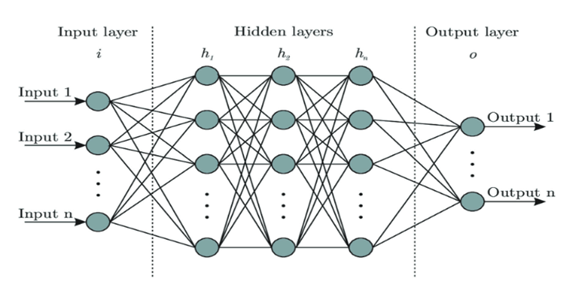
\includegraphics[scale=0.75]{NN_figure.png}
    \caption{Simple Neural Network Architecture. Adapted from \cite{https://doi.org/10.1002/cpe.6767}}
    \label{fig:my_label}
\end{figure}


Mathematically, a simple neural network with two hidden layers can be represented by the equations shown below, where \emph{h} is a layer, and \emph{y} is the output of the final activation function with respect to the previous layer. In this case, the hidden layers are called fully-connected or dense layers since the neuron units are directly connected to the previous layer’s neurons \cite{grosse2019lecture03}.
\newline
\newline
\centerline{$h{^(^1^)}_{i} = \phi^{^(^1^)}(\sum_{j} w_{ij}{^(^1^)}x_j{^(^1^)} + b_i{^(^1^)})$}

\centerline{$h{^(^2^)}_{i} = \phi^{^(^2^)}(\sum_{j} w_{ij}{^(^2^)}h_j{^(^1^)} + b_i{^(^2^)})$}

\centerline{$y_{i} = \phi^{^(^3^)}(\sum_{j} w_{ij}{^(^3^)}h_j{^(^2^)} + b_i{^(^3^)})$ \cite{grosse2019lecture03}}




\subsection{Convolutional Neural Networks}
CNNs are a commonly employed deep learning architecture, particularly in computer vision applications, that use the mathematical convolution operations in its layers \cite{grosse2019lecture09}. Traditional CNN architectures comprise of an input layer and one or more convolution and pooling layers followed by dense layers through to the output layer \cite{amidi_amidi}. Convolution layers apply mathematical convolution operations paired with a non-linear activation function to facilitate feature detection from an input signal \cite{grosse2019lecture09}. The layer hyperparameters include filter size (or kernel) and stride length \cite{amidi_amidi}. The resulting layer output is a feature map.  The activations for convolutional layers are computed where the feature maps, \emph{z}, are the sum of input \emph{x} convoluted by an input-output specific filter \emph{w}, with an element-wise activation function, $\phi$, applied as in the equations below. In contrast to dense layers, convolution layers are sparsely connected and employ weight sharing. Effectively reducing the number of necessary weights and connections for improved computation efficiency \cite{grosse2019lecture09}.
\newline
\newline
\centerline{$z_{i} = \phi^{^(^1^)}(\sum_{j} x_{j}*w_j)$}
\centerline{$h_i = \phi(z_i)$ \cite{grosse2019lecture09}}
\newline

Pooling layers are applied following the convolution layers to downsample the outputted feature maps, generally taking the maximum or average over a particular region of an input mapping \cite{grosse2019lecture09,amidi_amidi}. By taking the maximum value, the pooling layer can reduce the number of parameters and computational requirements without sacrificing the integrity of the detected features. Specifically, using the stride length \emph{S} as a hyperparameter, pooling layers reduce each dimension of the input representation by a factor \emph{S} \cite{grosse2019lecture09}. Pooling layers provide network architectures with the invariance properties with respect to input transformations, meaning that shifting network inputs slightly will not cause significant variations in classification decisions \cite{grosse2019lecture09}. 

\subsection{Activation Functions}
Activation functions are critical to generating the output of neurons, effectively defining the mathematical characteristics of the neural network \cite{lederer2021activation}. Specifically, the activation function’s derivatives and gradients are essential to training a neural network, particularly when computing hyperparameter optimizations. Common activation functions include logistic Sigmoid, Tanh, ReLU, and Softmax.

Sigmoid functions are smooth curves with one inflection point bound to a defined interval. Logistic Sigmoid activation functions are commonly employed in neural networks, mainly since it provides a smooth approximation of a binary function, also called a step-function \cite{lederer2021activation}. 
\newline
\newline
\centerline{$\sigma(z)=1/(1+exp(-z))$ \cite{lederer2021activation}}
\newline

For hidden layers, logistic Sigmoid functions, shown above, can be detrimental to a network’s training because of the saturation of values across the domain. In particular, the function lacks sensitivity when the input is very large or negative, making gradient-based learning computationally challenging for networks \cite{Goodfellow-et-al-2016}. It is only sensitive at the mid-point. Additionally, the function is known to struggle with the vanishing gradient problem during network backpropagation, leading to further challenges for multi-layer networks in training as layers are unable to update their parameters effectively. For this reason, logistic Sigmoid functions are not generally used for hidden layer activations. Instead, they are employed more frequently for output units, since applying a loss function at the final layer can effectively mitigate the impact of the inherent saturation issue \cite{Goodfellow-et-al-2016}. 

The hyperbolic tangent function, Tanh, shown below, is another type of Sigmoid function with similar properties to the logistic Sigmoid function. In essence, the Tanh function is “a shifted and scaled version” of the logistic Sigmoid function \cite{lederer2021activation}. Tanh functions, however, generally perform better than the logistic function in training neural networks, and, as such, are the preferred Sigmoid activation function \cite{Goodfellow-et-al-2016}. 
\newline
\newline
\centerline{$tanh(z) = \frac{e^{z} - e^{-z}}{e^{z} + e^{-z}}$ \cite{lederer2021activation}}
\newline

The ReLU (Rectified Linear Unit) function, shown below, is frequently used because of the simplicity of its implementation and gradients allow for easy optimization and reduced computation requirements \cite{lederer2021activation,Goodfellow-et-al-2016}. It is highly similar to a linear unit, however, the rectification zeros the output for half the domain, keeping gradients consistently large upon activation \cite{Goodfellow-et-al-2016}. This activation has its own form of a vanishing-gradient problem where many units may be inactive during training, which is especially detrimental when dealing with high complexity models \cite{lederer2021activation}.
\newline
\newline
\medskip
\centerline{$ReLU(z) = max(0,z)$ \cite{lederer2021activation}}
\newline

The Softmax regression function, shown below, is used in multi-class classification tasks for output layer units, calculating the likelihood of each target class over all classes. It is based on the logistic Sigmoid function, which maps the class probabilities to a binary output, but is modified to suit multiple classes \cite{unsupervised}.

\newline
\newline
\centerline{${Softmax}(z_{i}) = \frac{\exp(z_i)}{\sum_j \exp(z_j)}$ \cite{Goodfellow-et-al-2016}}
\newline

We note that for output layers, it is common to use Sigmoid or Softmax activation functions to define the final output for classification problems. Softmax is commonly employed in multi-class classification, while Sigmoid is well suited to multi-label classification problems where outputs are not mutually exclusive \cite{draelos_2019}.

\subsection{Loss Functions}
Cost functions are essential to gradient-based learning in neural networks, specifically by providing a measure to minimize during training for optimization processes. The cost function provides a metric to quantify the difference between predicted or estimated values and actual values. In gradient-based learning, the cost function is iteratively optimized by approximating its gradients where it may not be feasible computationally otherwise \cite{Goodfellow-et-al-2016}. Among the most common cost functions is the negative log-likelihood loss, which is particularly useful in classification problems \cite{NEURIPS2019_9015,nllloss}, shown in the equation below. The maximum likelihood estimation will be yielded upon minimizing negative log-likelihood loss. The trained neural network will select the highest probability target class as the resulting prediction \cite{Goodfellow-et-al-2016}.
\newline
\newline
\centerline{$NLL(y) = -{\log(p(y))}$ \cite{zhang}}
\newline



\subsection{Optimization Algorithms}
Optimizers are used to minimize loss functions during neural network training processes, effectively improving model performance through internal parameter updates \cite{8862686}. Specifically, parameter updates are performed once backpropagation is completed such that the gradient is fully completed. Among the most common optimizers are Stochastic Gradient Descent (SGD), AdaGrad, RMSProp, and Adam.  

SGD is a well-known optimization algorithm where the parameter update occurs by following the negative gradient direction such that the loss function is being minimized \cite{8862686,cs231n}. The gradient effectively describes the direction to follow such that the minimum of the loss function will be approached quickly. The update process utilizes the learning rate ($\alpha$) multiplied by the gradient to iteratively adjust parameters ($\theta$) until convergence \cite{8862686}, as shown in the formula below.
\newline
\newline
\centerline{$\theta_{i+1} = \theta_i - \alpha \nabla_\theta L$ \cite{price_wong_yuan_mathews_olorunniwo_2020}}
\newline
\newline
AdaGrad is an algorithm that provides adaptive learning rates for training neural networks. It reduces the advancement towards the loss function minima over time by computing the parameter-wise sum of squared gradients to normalize the update step \cite{8862686,cs231n}. As a result, the learning rates are adjusted based on how large a parameter’s gradient is, meaning that parameters with larger gradients will have the learning rate reduced or increased in the case of smaller ones \cite{cs231n}. The update rule is shown below as
\newline
\newline
\centerline{
$\theta_{i+1} = \theta_i - \alpha g_t/ \sqrt{\sum_{i=1}^t g_t^2}$ \cite{kingma2014adam}}

where $g_t$ is the gradient of the loss function.
\newline

RMSProp, which stands for Root Mean Square Propagation, relies on an exponentially weighted average of gradients, instead of the gradients computed each training epoch, to compute the parameter updates. It is, in essence, a less aggressive form of the AdaGrad optimizer \cite{8862686,cs231n}. The formula below describes the parameter update, with $E[g^2]_t$ as the moving average of gradients.
\newline
\newline
\centerline{
$\theta_{t+1} = \theta_t - {{\alpha}g_{t}/{\sqrt{E[g^2]_t}}}  $ \cite{huang_2020}}

The Adam optimizer is often recommended as a default algorithm due to its robust experimental performance \cite{cs231n}, as it provides an efficient stochastic gradient descent using adaptive estimation derived from the first and second order gradient moments \cite{cs231n}. It is essentially a mixture of the RMSProp and AdaGrad methods described in detail above, with a better ability to generalize performance \cite{cs231n,ajagekar_2021}. The core difference being that Adam uses the average of the second order gradient moments to compute the parameter updates, while RMSProp uses first order \cite{ajagekar_2021}. The parameter update rule is given by the equation below, where $\hat{a_t}$ is the bias-corrected first moment estimate and $\hat{v_t}$ is the bias-corrected second moment estimate.
\newline
\newline
\centerline{$\theta_{t+1} = \theta_t - {{\alpha}\hat{a_t}/(\sqrt{\hat{v_t}} + \epsilon}) $ \cite{kingma2014adam}}


\section{Data Collection and Pre-Processing}
To build our dataset, we collected 85 images, 46 of which were Eastern cottontail rabbits and 39 European hares, respectively. The images are labelled under one of two categories, \emph{rabbit} or \emph{hare}, with respect to the appropriate species to frame the single-label, multi-class classification task. Evidently, the class distribution is slightly unbalanced in favour of rabbits. The images were scraped from the internet through direct access via URL and saved in either the ‘.jpg’ or ‘.png’ format. To ensure that the dataset does not contain duplicate images, the \emph{difpy} \cite{landman} library was employed to automate the checking process through numerical analysis.

In collecting the dataset, we ensured that all instances contained only a single subject (i.e., one animal). However, we note that the background environments and subjects’ positioning vary among samples. In particular, the background colour variations indicated that considerations in pre-processing the data may be necessary to generalize the model better, and to ensure that the model instead focuses on the subject’s key features. 

For data pre-processing, the image encoding pipeline consisted of five steps employing the CV2 library \cite{opencv_library} to streamline the process. First, images were scaled and resized concerning the original aspect ratio to reach the target dimensions of 200 by 200 pixels. Next, the images were converted to greyscale using CV2.cvtColor to transform from the RGB colour space using the array conversion as shown in the equation below \cite{opencv_library}. 
\newline
\newline
\centerline{$\text{RGB[A] to Gray:} \quad Y \leftarrow 0.299 \cdot R + 0.587 \cdot G + 0.114 \cdot B$ \cite{opencv_library}}

Once converted, the images were normalized using CV2.normalize with MinMax normalization, with alpha and beta set to 0 and 1, respectively. Numerically, the normalization scales the image array elements such that the pixel values fall between the upper boundary (beta) and lower boundary (alpha), as depicted in the equation below. This process effectively reduces noise in the data and the dimensionality, which in turn proves helpful in improving convergence while training the model \cite{opencv_library}.
\newline
\newline
\centerline{$\min _I \texttt{dst} (I)= \texttt{alpha} , \, \, \max _I \texttt{dst} (I)= \texttt{beta}$ \cite{opencv_library}}

Finally, the normalized images are padded and cropped to ensure uniformity before being passed to the model's input layer with a 200 by 200 shape. With respect to the label pre-processing, we employed label-encoding encoding using the scikit-learn \cite{scikit-learn} pre-processing module to create unique binary labels for the data categories, as is standard in classification problems.

\section{Model Architectures}
To receive valuable results from our experimentation, we first had to develop a baseline model that they could be built from. Creating this neural network was an iterative process in which we intended to create a model that performed adequately, with room for improvement through experimentation. At the end of this process, we had created a model with three convolution layers of increasing filter quantity and a dropout layer prior to the dense layer. This provided us with baseline training, validation, and testing accuracy of 0.91, 0.69 and 0.53 respectively. With the metrics obtained from this model, we were able to evaluate the results from our experiments and gain a more significant measure of whether they positively or negatively impacted the network. Our baseline architecture is shown in Figure \ref{fig:CNN} below.
\newline
\begin{figure}[h!]
    \centering
    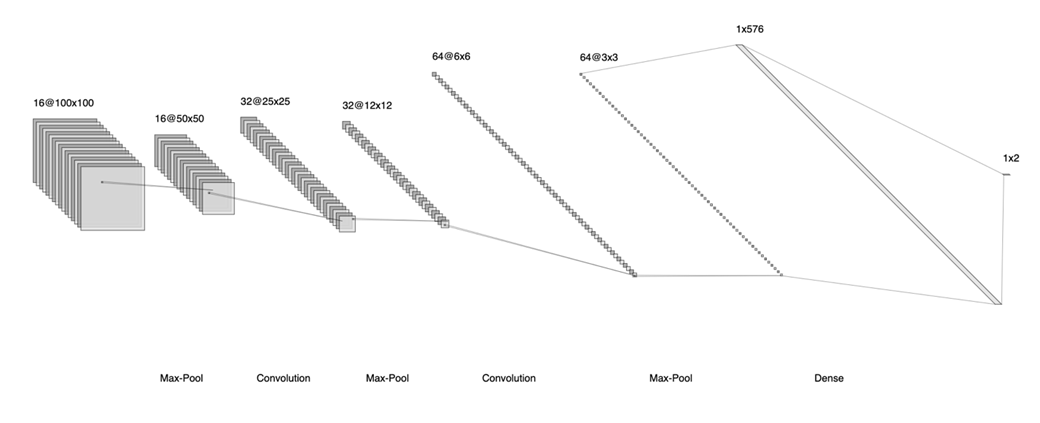
\includegraphics[scale=0.65]{CNN.png}
    \caption{Lepus Classifier Baseline CNN Architecture}
    \label{fig:CNN}
\end{figure}


\section{Experiments and Analysis}
 We explore the design and training process of an image classification neural network, looking to neural network architecture changes and hyperparameter tuning for the core of our experiments. We implement the CNN using Pytorch \cite{NEURIPS2019_9015} and Pytorch Lightning \cite{pytorch-lightning} frameworks. Additionally, we experiment with training algorithms and optimizations. The sections below explore training the CNN using Stratified K-Fold Splitting and various optimization algorithms. We explore modifying convolution layers through the experimentation of the number of convolutions, the depth of the network, the width of the network, and pooling methods, as well as consider the implications of dropout layers. Additionally, we consider the performance impact of different activation functions. The full results for our experiments can be found in the appendixes at the end of this report, as well as on our code repository and \emph{Weights \& Biases} \cite{wandb} project for full trial logs (Appendix A). 

\subsection{Stratified K-Fold Split}
Small and unbalanced data sets, such as ours, often result in models that poorly fit the input, have selection bias or both. As a result, it was deemed necessary to find alternative sampling and training strategies to prevent the fore-mentioned problems.

\subsubsection{Stratified Sampling}
Stratified sampling is a sampling method in which each selected batch of inputs shares the same percentage of selected entities across all classes. In other words, stratified sampling ensures that a class will have contributed to the learning process during the fitting stage \cite{scikit-learn}.

\subsubsection{K Fold Cross Validation}
K-fold cross-validation is a fitting strategy that breaks the data set into $K$ even subsets, where one subset is left out (the validation set) and, the remaining subsets are utilized during training. With each fold iteration, a new subset is left out until all subsets have been used during validation. The prime advantage of this strategy over a typical train-test split is that it ensures that all training data is used \cite{scikit-learn}. As networks with more data typically outperform networks with large amounts of data, it is essential that as much data as possible is retained during fitting.

\subsubsection{Analysis}
The use of k-fold cross-validation offers better performance than a typical train-test split strategy. As demonstrated in Table \ref{table:kfold}, as the numbers of folds approached 3, the metrics improved. It should be noted that K-Fold/1 is treated as the baseline and consists of using the \emph{StratifiedShuffleSplit} module with a training/validation ratio of 80:20 \cite{scikit-learn}. This is likely because an insufficient number of folds can result in the unbalanced class being absent during training, whereas an abundance of folds results in the unbalanced class not having enough samples provided during training.


\subsection{Batch Size}
Batch sizes indicate the number of images used to estimate the network’s gradients while training \cite{KANDEL2020312}. Based on the size of our dataset, we opted to experiment with relatively smaller batch sizes. Specifically, we consider batch sizes of 2, 4, 8, 16, and 32 for training with our baseline CNN model for a maximum of 100 epochs. These batch sizes were selected to be powers of 2 to take advantage of GPU architecture for improved performance in training. Smaller batch sizes allow for faster convergence and a regularization effect due to high variance during training. However, reaching an optimum minimum may not be possible \cite{KANDEL2020312}. 

The results of these experiments are shown in Table \ref{table:batch} in Appendix B. We observed that the best performance came from using a batch size of 2, yielding training, testing, and validation accuracies of 1.0, 0.53, and 0.77, respectively. We note a significant drop in model performance for batch sizes 16 and 32, where the training accuracies drop to below 0.8 and training loss remains above 0.25. Interestingly, the model with batch size 32 achieves a high validation accuracy of 0.77. However, it fails to accurately predict the test set with an accuracy of only 0.47. While batch sizes 4 and 8 achieve comparable training and test results to the model using a batch size of 2, with scores above 0.9 and 0.53, respectively, both models' performances suffer in validation tests. We note that the models fail to minimize the validation loss effectively, as they yield losses of 0.94 and 2.34, respectively. Thus, based on our results, a batch size of 2 appears to be the appropriate parameter selection for our task.

\subsection{Optimizers}

While all of the optimizers achieved similar performance, as seen in Table \ref{table:optim}, the SGD optimizer with momentum was able to generalize the model better. Likely due to the initial small learning rate, using an adaptive optimizer resulted in training to slow down significantly. In the process, the models could probably not derive adequate information from each batch.

\subsection{Dropout}

Our baseline model showed a divergence between training and validation accuracy over a certain number of steps per fold. While the training accuracy would trend upwards towards 1, the validation accuracy would plateau and eventually decrease. This is due to the model learning the noise in the training image data, which led to poor generalization across the validation and testing datasets. To mitigate this effect, we increased the drop rate. We expanded the number of dropout layers throughout several experiments to observe its regularizing impact on the model’s metrics. Dropout regularization could make the model more robust through the random dropping of layer outputs (controlled by a drop rate hyperparameter). This effectively simulates the combining of several neural nets and reduces the co-adaptation between nodes that do not generalize \cite{JMLR:v15:srivastava14a}. 

In our first two experimental models, as displayed in Table \ref{table:drop}, we increased the drop rate of our dropout layer from the baseline of 0.2 to 0.4 (Drop01) and then to 0.5 (Drop02). Across these three models, we saw an explainable decrease in training accuracy, from 0.91 to 0.89 and then 0.82, due to the model’s shrinking capacity to memorize information in the training dataset. Of these three models, we noted a maximum validation accuracy of 0.77 for Drop02, which possessed a drop rate of 0.5, a commonly used value. We also added an additional dropout layer after the second convolution layer (Drop03) to continue this trend. However, for this model, the training accuracy and validation accuracy both dropped to 0.65 and 0.69, respectively. Though the gap between these two values had reduced, the information loss from the dropout layers reduced the model’s capacity to label the image data accurately.

\subsection{Pooling}

For this experiment, we wanted to examine the impact of average pooling layers on the accuracy of the model, in comparison to the max pooling layers utilized in the baseline model. The outcome of the average pooling model (Pool01), visible in Table \ref{table:pool}, was a significant decrease in training accuracy in comparison to the baseline model (from 0.91 to 0.69) but also a significant increase in validation accuracy (from 0.69 to 0.85). The test accuracy remained barely impacted, dropping from 0.53 to 0.47. This is indicative that the average pooling model generalized better from the training data to the validation data than the max pooling baseline model. We believe that this was due to the max-pooling model highlighting features that were irrelevant to the classification of the image, such as bright elements in the background, leading to the memorization of the training set. The more greater representation of all elements in the model through average pooling may have led to this increase in validation accuracy.

\subsection{Convolutions}

In an attempt to increase validation and testing accuracy, we decided to evaluate the impact of kernel size and stride length on our model. For our baseline, the convolution layers utilized a 2x2 kernel size and a stride value of 2. We decided to, over the course of several models, measure the impact of increasing kernel size and decreasing stride length. We knew that increasing the kernel size would also increase the number of parameters in the model, possibly improving the models ability to recognize valuable information in the image data. We then decreased the stride length from 2 to 1, which would increase the size of the feature maps and reduce any potential loss of information from a larger stride length \cite{Goodfellow-et-al-2016}.

As seen in Table \ref{table:convolution}, upon the increase of the kernel size in the first experimental model (Convolution01), we noted a raise in training accuracy from 0.91 to 1.0 and a fall in validation accuracy from 0.69 to 0.61, while testing accuracy remained unchanged. In the second model (Convolution02), training and testing accuracy remained constant at 1.0 and 0.53 respectively, however the validation accuracy increased to 0.76. This gap between the training and validation accuracy is indicative of the model overfitting, which is explainable due to the increased number of parameters reducing the model's ability to generalize to the validation and test image sets.

\subsection{Depth}

To further improve the model's predictive capacity, we determined that we should experiment with the depth of the model. We believed that through expanding the amount of layers in the model, the additional parameters and increased filter size may be able to decipher more advanced pattern information that would assist in classification \cite{Goodfellow-et-al-2016}.

First we created a model (Depth01) which possessed an additional convolution layer and max pooling layer prior to the dense layer. As seen in Table \ref{table:depth}, in comparison to our baseline, the training accuracy increased to 1 in comparison to the baseline 0.91, while the validation accuracy also increased from 0.69 to 0.77. Test accuracy, however, decreased from 0.53 to 0.41. Similar to the previous convolutions experiment, we believe that the increased quantity of parameters led to over-fitting on the training set, raising it to 1 while diminishing the test accuracy. For the second model of this experiment (Depth02), we included an additional dropout layer with a drop rate of 0.5 after the final max pooling layer to mitigate the over-fitting. This resulted in an improved test accuracy from 0.41 to 0.47 and a reduction in training and validation accuracy to 0.91 and 0.69 respectively. It is clear the additional dropout layer reduced the memorization of the training set, however Depth02, with its greater quantity of parameters, does not improve any metric in comparison to the baseline model.

\subsection{Width}

The quantity of filters in a given convolution layer determines the number of different features that can be learned in parallel given an input \cite{inproceedings}. In order to increase validation and testing accuracy, we experimented with the quantity of filters in each convolution layer, believing that increasing this hyperparameter may enable the model to learn a greater number of valuable patterns to assist in classification.

In our experimental model (Width01), we doubled the baseline number of filters in each convolution layer. This model performed with a slightly reduced test accuracy of 0.47, visible in Table \ref{table:width}, but displayed an increased training and validation accuracy, similar to previous experiments in which we raised the quantity of parameters in the model. As formerly observed, the increased number of parameters in the model does not translate into the learning of generalized patterns between the two species, but instead the memorization of the training set.

\subsection{Hidden-Layer Activations}
In our experiments, we modify the activation functions of the hidden layers in our baseline CNN architecture to observe their impact on training and hyperparameter fine-tuning. We employ ReLU, Tanh, and logistic Sigmoid activation functions for this task since they are among the most used. We note that ReLU was selected as our default activation function for our baseline architecture due to the simplicity of its computational requirements.

The results of these experiments are shown in Table \ref{table:actfunc} in Appendix B. Using ReLU activations, the model achieved training, testing, and validation accuracies of 1.0, 0.53, and 0.92, respectively. We note a large discrepancy between the testing and validation scores. However, the model can minimize the loss function effectively enough. It is possible that the simplicity of the ReLU activation’s gradients may be causing a challenge in training a complex, feature-driven network to handle the Lepus data. With the Tanh activation, the network achieves a far more balanced performance than previous iterations, with training, testing, and validation accuracies of 1.0, 0.65, and 0.62, respectively. We note that the loss functions across all three sets are significantly minimized with Tanh activations than ReLU and logistic Sigmoid. Finally, with logistic Sigmoid, accuracies of 0.64, 0.47, and 0.62 across the train, test, and validation sets, the poorest performance in this set of experiments by a large margin. This behaviour is not unexpected based on the mathematical characteristics of this function, as discussed in Section 2.3. Based on the performance in these experiments, Tanh activation trains a more consistent, well-rounded network that can capture the complexity of the Lepus data more effectively.

\subsection{Final Model}

Based on the experiments conducted in previous sections where we modified the CNN architecture and fine-tuned parameters, we established a final model using PyTorch Lightning \cite{pytorch-lightning} for the Lepus Classifier. The model architecture is shown in Table \ref{table:final_model} below in Appendix B. We employed stratified 3-fold cross-validation for training using an SGD optimizer with a batch size of 2 based on our previous performance results. 

The performance results of this final model are shown in Table \ref{table:final_results} in Appendix B. We observe that the training, testing, and validation accuracies are 0.65, 0.47 and 0.73. These results are not ideal. However, they provide a solid baseline to consider in future work. While each component determined from the previous experiments helped finalize an architecture and training process in this project's scope, we believe that re-adjusting the architecture development process to follow an iterative tuning process over a parallel one would benefit performance. We believe that extending the dataset would prove useful in improving model performance, such that the model would better capture the complexity of differentiating between the highly similar images of rabbits and hares. 


\section{Conclusion}

From our experimental findings, we have yielded promising results that would serve as a solid foundation for further expansion. Going forward, we would need to expand beyond the toy dataset of 85 images in order to build a more robust system. This is dependent on greater access to computational resources and time. Thus far, we have received valuable indications of the impact on model performance by several critical aspects of the model; however, better differentiation between hares and rabbits requires more feature learning from a larger quantity of data.


\bibliographystyle{IEEEtranN}
\bibliography{References}


\medskip


\appendix

\section{Appendix}
\subsection{Project Repository and Logs}
Lepus Classifier code repository: \url{https://github.com/urmzd/lepus-classifier}
\newline
Weights and Biases project: \url{https://wandb.ai/csci-4155-rabbit-classifier}
\newline
\section{Appendix}
\subsection{Experimental Results}

\begin{table}[h!]
\caption{Results for K Fold Cross Validation}
\label{table:kfold}
\begin{tabular}{@{}lllllll@{}}
\toprule
Name     & learning\_rate & test/Accuracy & test/F1Score & test/Precision & test/Recall & test/loss \\ \midrule
K-Fold/5 & 0.02           & 0.588235      & 0.564103     & 0.591667       & 0.576389    & 0.568222  \\
K-Fold/4 & 0.02           & 0.470588      & 0.463158     & 0.464286       & 0.465278    & 0.487269  \\
K-Fold/3 & 0.02           & 0.647059      & 0.575        & 0.8            & 0.625       & 0.010687  \\
K-Fold/2 & 0.02           & 0.647059      & 0.575        & 0.8            & 0.625       & 0.3403    \\
Baseline & 0.02           & 0.588235      & 0.582456     & 0.585714       & 0.583333    & 3.669271  \\ \bottomrule
\end{tabular}
\end{table}

\begin{table}[h]
    \centering    
    \caption{Experimental results for batch size parameter}
    \label{table:batch}
    \begin{tabular}{llll}
        \toprule
        \centering
        {Batch Size} & train accuracy & test accuracy & validation accuracy \\
        \midrule
         2 & 1.00  & 0.53 & 0.77 \\
         4 & 0.98 & 0.53 & 0.54  \\
         8 & 0.93 & 0.53 & 0.69 \\
         16 & 0.76 & 0.53 & 0.69 \\
         32 & 0.78 & 0.47 & 0.77 \\
        \bottomrule
    \end{tabular}
\end{table}

\begin{table}[h!]
    \centering
    \caption{Experimental results for optimizer}
    \label{table:optim}
    \begin{tabular}{lllllll}
        \toprule
            Name    & learning\_rate & momentum & test/Accuracy & test/F1Score & test/Precision & test/Recall \\ \midrule
            Adam    & 0.00001        &          & 0.411765      & 0.291667     & 0.233333       & 0.388889    \\
            RMSprop & 0.00001        &          & 0.411765      & 0.291667     & 0.233333       & 0.388889    \\
            SGD     & 0.00001        & 0.99     & 0.470588      & 0.463158     & 0.464286       & 0.465278    \\
            AdaGrad & 0.00001        &          & 0.470588      & 0.32         & 0.25           & 0.444444  \\ 
        \bottomrule
    \end{tabular}
\end{table}

\begin{table}[h!]
    \centering    
    \caption{Experimental results for dropout}
    \label{table:drop}
    \begin{tabular}{llll}
        \toprule
        \centering
        {Dropout Variation} & train accuracy & test accuracy & validation accuracy \\
        \midrule
         Baseline w/ drop rate of 0.2 & 0.91  & 0.53 & 0.69 \\
         Baseline w/ drop rate of 0.4  & 0.89 & 0.41 & 0.62  \\
         Baseline w/ drop rate of 0.5 & 0.82 & 0.47 & 0.77 \\
         Baseline w/ additional dropout layer & 0.65 & 0.47 & 0.69 \\
        \bottomrule
    \end{tabular}
\end{table}

\begin{table}[h!]
    \centering    
    \caption{Experimental results for pooling experiments}
    \label{table:pool}
    \begin{tabular}{llll}
        \toprule
        \centering
        {Pooling Type} & train accuracy & test accuracy & validation accuracy \\
        \midrule
         Max Pooling & 0.91  & 0.53 & 0.69 \\
         Average Pooling  & 0.69 & 0.47 & 0.85  \\
        \bottomrule
    \end{tabular}
\end{table}

\begin{table}[]
    \centering    
    \caption{Experimental results for convolution layer experiments}
    \label{table:convolution}
    \begin{tabular}{llll}
        \toprule
        \centering
        {Convolution Layer Setup} & train accuracy & test accuracy & validation accuracy \\
        \midrule
         Kernel Size = 2; Stride = 2 & 0.91  & 0.53 & 0.69 \\
         Kernel Size = 3; Stride = 2 & 1.00 & 0.53 & 0.62  \\
         Kernel Size = 3; Stride = 1 & 1.00 & 0.53 & 0.77  \\
        \bottomrule
    \end{tabular}
\end{table}

\begin{table}[ht!]
    \centering    
    \caption{Experimental results for depth experiments}
    \label{table:depth}
    \begin{tabular}{llll}
        \toprule
        \centering
        {Architecture Setup} & train accuracy & test accuracy & validation accuracy \\
        \midrule
         3 Convolution Layers; 3 Pooling Layers; 1 Dropout Layer & 0.91  & 0.53 & 0.69 \\
         4 Convolution Layers; 4 Pooling Layers; 1 Dropout Layer & 1.00 & 0.41 & 0.77  \\
         4 Convolution Layers; 4 Pooling Layers; 2 Dropout Layers & 0.91 & 0.47 & 0.69  \\
        \bottomrule
    \end{tabular}
\end{table}

\begin{table}[ht!]
    \centering    
    \caption{Experimental results for width experiments}
    \label{table:width}
    \begin{tabular}{llll}
        \toprule
        \centering
        {Architecture Setup} & train accuracy & test accuracy & validation accuracy \\
        \midrule
         Convolution Layers w/ Filter Quantities 16, 32 and 64 & 0.91 & 0.53 & 0.69 \\
         Convolution Layers w/ Filter Quantities 32, 64 and 128 & 1.00 & 0.47 & 0.77 \\
        \bottomrule
    \end{tabular}
\end{table}

\begin{table}[ht!]
    \centering    
    \caption{Experimental results for hidden layer activation functions}
    \label{table:actfunc}
    \begin{tabular}{llll}
        \toprule
        \centering
        {Activation Function} & train accuracy & test accuracy & validation accuracy \\
        \midrule
         ReLU & 1.00  & 0.53 & 0.92 \\
         Tanh & 1.00 & 0.65 & 0.62  \\
         Sigmoid & 0.64 & 0.47 & 0.62 \\
        
        \bottomrule
    \end{tabular}
\end{table}

\begin{table}[!ht]
    \centering
    \label{table:final_model}
    \caption{Final Model architecture}
    \begin{tabular}{@{}llll@{}}
    \hline
        \toprule
        Layer & Parameters & Output Shape & No. of Parameters \\ \midrule
        Conv2d(1, 16, kernel\_size=(3, 3), stride=(1, 1)) & weight,16,1,3,3,bias,16 & 2,16,198,198 & 144,16 \\
        AvgPool2d(kernel\_size=2, stride=2, padding=0) & ~ & 2,16,99,99 & ~ \\ 
        ReLU() & ~ & 2,16,99,99 & ~ \\ 
        Conv2d(16, 32, kernel\_size=(3, 3), stride=(1, 1)) & weight,32,16,3,3,bias,32 & 2,32,97,97 & 4608,32 \\ 
        AvgPool2d(kernel\_size=2, stride=2, padding=0) & ~ & 2,32,48,48 & ~ \\ 
        ReLU() & ~ & 2,32,48,48 & ~ \\ 
        Conv2d(32, 64, kernel\_size=(3, 3), stride=(1, 1)) & weight,64,32,3,3,bias,64 & 2,64,46,46 & 18432,64 \\ 
        AvgPool2d(kernel\_size=2, stride=2, padding=0) & ~ & 2,64,23,23 & ~ \\ 
        ReLU() & ~ & 2,64,23,23 & ~ \\
        Dropout2d(p=0.5, inplace=False) & ~ & 2,64,23,23 & ~ \\ 
        Flatten(start\_dim=1, end\_dim=-1) & ~ & 2,33856 & ~ \\ 
        Linear(in\_features=33856, out\_features=2, bias=True) & weight,2,33856,bias,2 & 2,2 & 67712,2 \\
        LogSoftmax(dim=None) & ~ & 2,2 & ~ \\
        \bottomrule
    \end{tabular}
    \label{table:final_model}
\end{table}

\begin{table}[!ht]
    \centering    
    \caption{Experimental results for the Final Model}
    \label{table:final_results}
    \begin{tabular}{llll}
        \toprule
        \centering
        {} & train accuracy & test accuracy & validation accuracy \\
        \midrule
         Final Model & 0.65  & 0.47 & 0.73 \\
        \bottomrule
    \end{tabular}
\end{table}





\end{document}